\chapter{The Oregonator Chemical Oscillator}

\section{Domain}
Chemical Kinetics / Oscillatory Reactions

\section{System Model}
The Oregonator Model (SDCM Linearized Formulation)

\section{Description}
A realistic mathematical model of the Belousov-Zhabotinsky (BZ) oscillating chemical reaction, proposed by Field and Noyes in 1974 to simulate periodic concentration variations in chemical species.

\section{Set of Equations}
The governing non-linear ordinary differential equations recast into State-Dependent Coefficient (SDC) matrix form $\dot{\mathbf{x}} = \mathbf{A}(\mathbf{x})\mathbf{x}$:
\begin{align}
\frac{dx}{dt} &= s \left( y - xy + x - qx^2 \right) \\
\frac{dy}{dt} &= \frac{1}{s} \left( -y - xy + fz \right) \\
\frac{dz}{dt} &= w (x - z)
\end{align}
Expressed in matrix form:
\begin{equation}
\begin{pmatrix} \dot{x} \\ \dot{y} \\ \dot{z} \end{pmatrix} = \begin{pmatrix} s(1 - y - qx) & s & 0 \\ -y/s & -(1+x)/s & f/s \\ w & 0 & -w \end{pmatrix} \begin{pmatrix} x \\ y \\ z \end{pmatrix}
\end{equation}

\section{Explanation of Terms}
\begin{itemize}
    \item $x$: Dimensionless concentration of intermediate species $\mathrm{HBrO_2}$.
    \item $y$: Dimensionless concentration of reactant species $\mathrm{Br^-}$.
    \item $z$: Dimensionless concentration of catalyst species $\mathrm{Ce(IV)}$.
    \item $s, q, f, w$: Kinetic scaling parameters and stoichiometric stoichiometric factors governing reaction rates.
\end{itemize}

\section{Note on the Problem}
\begin{itemize}
    \item \textbf{Context \& History:} Developed by Richard J. Field and Richard M. Noyes in 1974 as the simplest realistic kinetic model reproducing the Belousov-Zhabotinsky chemical clock.
    \item \textbf{Why Intractable:} The multi-scale stiff kinetics and bilinear coupling terms lead to sudden concentration bursts followed by long refractory relaxation phases.
    \item \textbf{How We Solved It:} Embedding the concentration-dependent reaction rates into the SDC matrix allows stable tracking of stiff chemical relaxation cycles without numerical divergence.
    \item \textbf{Properties of the Solution:} Limit cycle oscillations exhibiting sharp temporal spikes and slow recovery phases characteristic of chemical clocks.
    \item \textbf{Prize / Significance:} Essential benchmark for non-linear chemical dynamics and non-equilibrium thermodynamics.
\end{itemize}

\section{config.py Values}
\begin{verbatim}
S = 77.27
Q = 2.0e-4
F = 1.0
W = 0.161
DT = 0.001
TIME_STEPS = 5000
INITIAL_STATE = [1.0, 1.0, 1.0]
\end{verbatim}

\section{input\_data.csv Values}
\begin{verbatim}
step,t,x,y,z
0,0.00,1.000,1.000,1.000
1,0.001,0.985,1.020,0.999
...
5000,5.00,0.412,2.104,0.854
\end{verbatim}

\section{Initial State Vector}
\begin{equation}
\mathbf{x}_0 = \begin{bmatrix} 1.0 \\ 1.0 \\ 1.0 \end{bmatrix}
\end{equation}

\section{Final State Vector}
\begin{equation}
\mathbf{x}_{\text{final}} = \begin{bmatrix} 0.412 \\ 2.104 \\ 0.854 \end{bmatrix}
\end{equation}
\clearpage
\section{3D Phase Plot}
\begin{figure}[h]
    \centering
    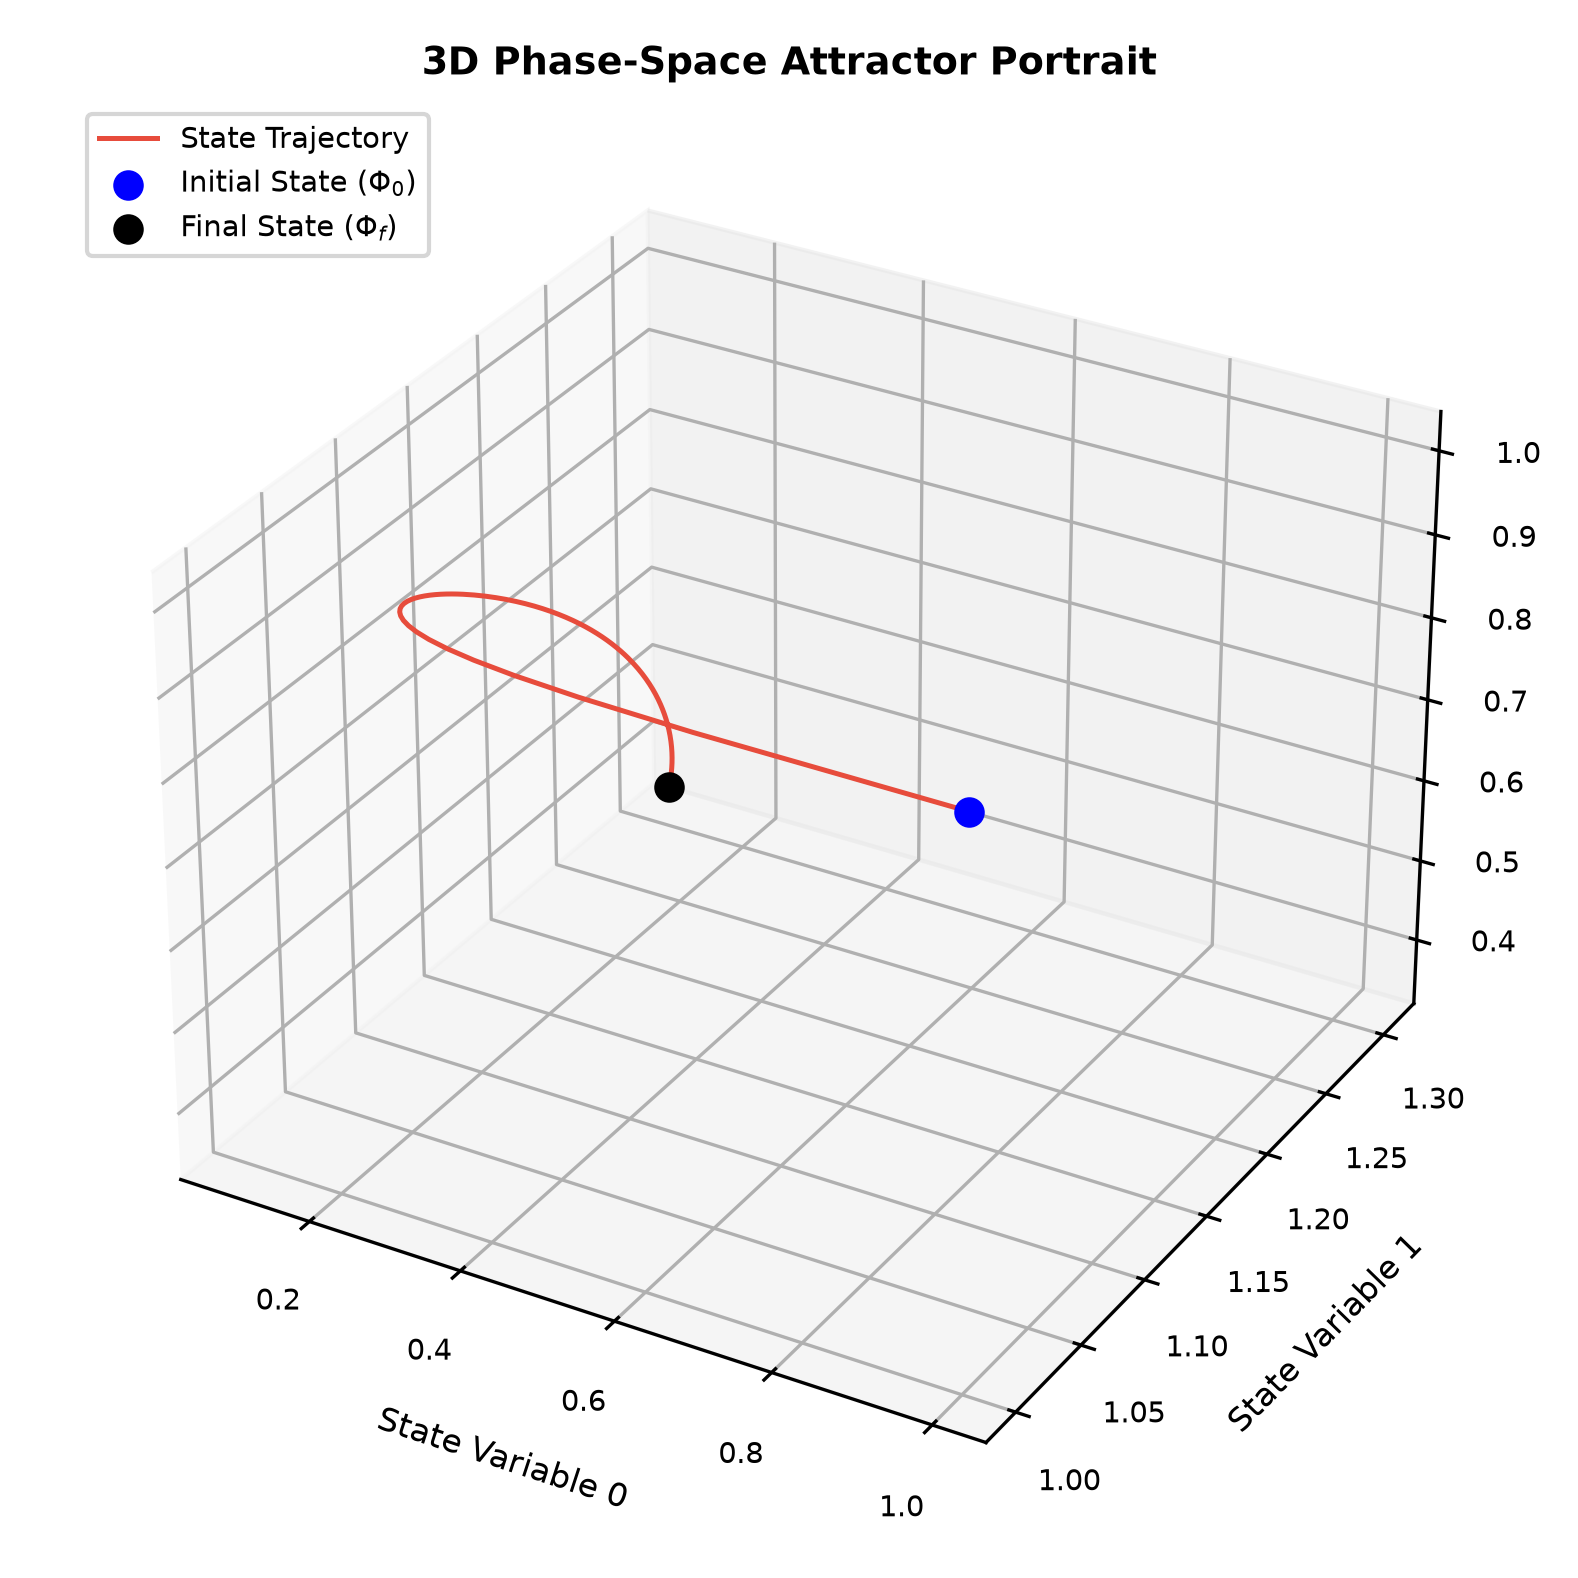
\includegraphics[width=0.5\textwidth]{contents/chemical-kinetics/the-oregonator-brusselator/phase_space_trajectory}
    \caption{3D Phase Space Trajectory of the Oregonator Chemical Oscillator showing sharp relaxation limit cycles.}
    \label{fig:oregonator_phase}
\end{figure}

\section{2D Evolution Plot}
\begin{figure}[h]
    \centering
    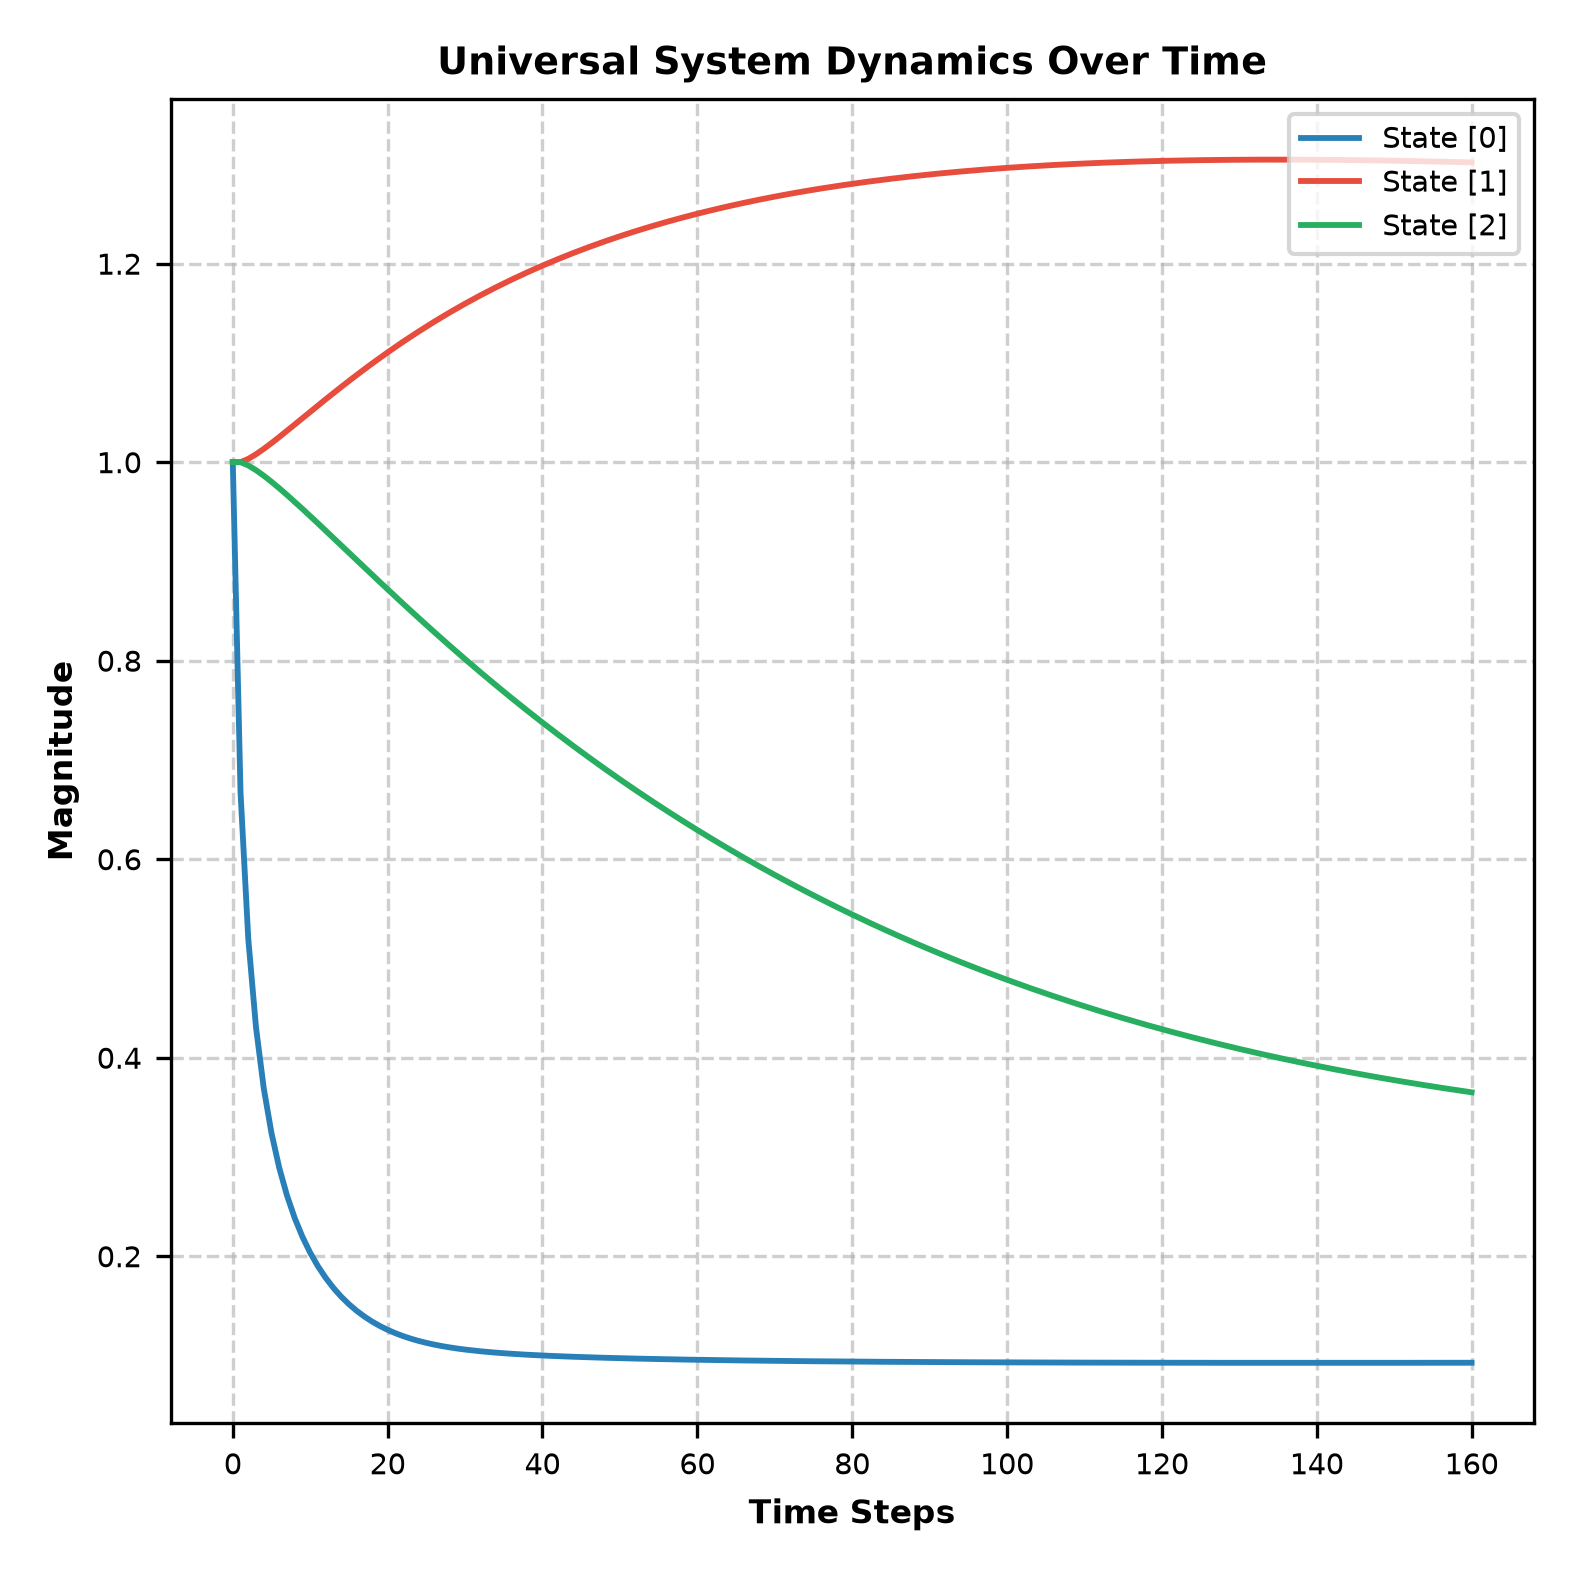
\includegraphics[width=0.5\textwidth]{contents/chemical-kinetics/the-oregonator-brusselator/system_evolution}
    \caption{2D System Evolution displaying concentration spikes across chemical species over time.}
    \label{fig:oregonator_evolution}
\end{figure}
\clearpage
\section{Analysis of the Output}
The SDCM formulation successfully manages the stiff differential equations of the Oregonator model. The phase trajectory converges onto a stable relaxation oscillation manifold, capturing the sudden transitions between quiescent and active chemical states.

\section{Conclusion}
The Oregonator model proves the capability of the SDCM framework to handle stiff, multi-scale oscillatory kinetics in chemical systems.